\documentclass[11pt,letterpaper]{report}

\usepackage[utf8]{inputenc}
\usepackage[T1]{fontenc}
\usepackage[spanish,provide=*]{babel}
\usepackage{amsmath,amssymb}
\usepackage{booktabs}
\usepackage{array}
\usepackage{longtable}
\usepackage{multirow}
\usepackage{graphicx}
\usepackage{float}
\usepackage{caption}
\usepackage{tikz}
\usepackage{pgfplots}
\pgfplotsset{compat=1.17}
\usetikzlibrary{arrows.meta}
\usepackage[margin=2.5cm]{geometry}
\usepackage{enumitem}
\usepackage{siunitx}

\newcommand{\Prob}{\operatorname{Prob.}}
\newcommand{\E}{\operatorname{E}}
\newcommand{\VAR}{\operatorname{VAR}}
\renewcommand{\arraystretch}{1.15}

\begin{document}

\begin{center}
{\LARGE\bfseries\linespread{1.3}\selectfont 5. APLICACIONES DE SIMULACIÓN\par}
\end{center}
\vspace{0.5cm}

\setcounter{chapter}{5}
\setcounter{page}{67}

%==========================================================
\section*{Introducción}

En capítulos anteriores, se han explicado y analizado los conceptos y
herramientas requeridas por un estudio de simulación. Por consiguiente,
ahora ya estamos preparados para empezar a discutir el papel tan
importante que los modelos de simulación juegan en el análisis y estudio
de varios tipos de sistemas.

Los modelos de simulación presentan la ventaja de poder ser manipulados
en diferentes formas, que serían imposibles, imprácticas y demasiado
costosas si se realizaran a través de otra metodología. Por ejemplo, se
puede simular la operación de un sistema sin que éste aún exista, también
se puede a través del uso de simulación determinar el sitio de
localización de un almacén, determinar políticas óptimas de inventarios
cuando la demanda y el tiempo de entrega son estocásticos, etc. En
general, se puede decir que los modelos de simulación se usan para: 1)
Análisis de sistemas, 2) Diseño de sistemas, 3) Síntesis de sistemas y 4)
Entrenamiento.

El presente capítulo, tiene como objetivo presentar una serie de
ejemplos, a través de los cuales se podrá tener una idea de los múltiples
usos y de la utilidad que se puede obtener al utilizar la técnica de
simulación.

%==========================================================
\section*{Ejemplo 5.1. Juego de volados}

Existe un método viejo para jugar volados, que consiste en doblar la
apuesta cada vez que se pierde. Por ejemplo, si se apuesta \$X y se
pierde, entonces, se apuesta \$2X; si en esta ocasión se vuelve a perder,
entonces, se apuesta \$4X y así sucesivamente. Sin embargo, si al seguir
esta política sucede que la apuesta es mayor que la cantidad de que se
dispone, entonces, se apuesta lo que se tiene disponible. Por el
contrario, cada vez que se gane, la apuesta será de \$X. Si la cantidad
inicial disponible es de \$30, la apuesta es de \$10, la ganancia es igual
a la cantidad apostada, la probabilidad de ganar en un volado es 0.5 y se
quiere tener \$50, ¿cuál es la probabilidad de llegar a la meta?

Para la información anterior, la tabla 5.1 muestra los resultados de una
simulación manual para este juego de volados. Como se puede observar en
esta tabla, en la primera ``corrida'' se necesitaron dos lanzamientos
para llegar a la meta de tener \$50. El primer lanzamiento de esta corrida
el cual está representado por el número aleatorio 0.03991, significa que
se ganó en el volado (números aleatorios menores de 0.5 representan al
evento ganar, y números aleatorios mayores que 0.5 representan al evento
perder), y por consiguiente, la apuesta en el siguiente volado será de
\$10. Como el número aleatorio de este segundo volado es menor que 0.5,
entonces, con este lanzamiento se llega a la meta de \$50.

Por otra parte, la corrida número 3 representa una situación de quiebra,
es decir, esta corrida representa una situación en la que se pierde
completamente la cantidad inicial disponible. En esta corrida, se pierde
el primer volado, y por consiguiente, la apuesta del segundo volado es
\$20. Como el número aleatorio de este lanzamiento es menor que 0.5,
entonces, se gana en el segundo volado, y la apuesta del tercer volado
será de \$10. Como el número aleatorio de este volado es mayor que 0.5,
entonces, se pierde en el tercer volado, y la apuesta del cuarto volado
será de \$20. Puesto que el número aleatorio de este volado es mayor que
0.5, entonces, se pierde en el cuarto volado, y la apuesta será de \$40.
Sin embargo, la cantidad que se tiene al final del cuarto volado es de
\$10. Por consiguiente, la cantidad apostada en el quinto volado será de
\$10. Como esta cantidad es perdida en el último lanzamiento, entonces, se
llega finalmente a una situación de quiebra.

Finalmente, en esta tabla se puede observar que de 10 corridas, en 6
ocasiones se llegó a la meta. Esto significa que la probabilidad de llegar
a la meta es de 0.6. Sin embargo, es necesario señalar que esta estimación
no es muy confiable por el número tan reducido de corridas que se
simularon. Para tomar una decisión que garantice buenos resultados, es
necesario aumentar significativamente el número de corridas simuladas.
También, vale la pena mencionar que este problema sería demasiado difícil
de resolver analíticamente, sin embargo, a través del uso de simulación se
facilita tremendamente la estimación de la probabilidad buscada.

\begin{table}[H]
\centering
\caption*{\textbf{Tabla 5.1} Resultados de la simulación manual de un juego de volados}
\begin{tabular}{cccccccc}
\toprule
Número de & Cantidad antes & \multirow{2}{*}{Apuesta} & Número$^{*}$ & ¿Se ganó & Cantidad después & ¿Se llegó \\
corrida & del volado & & aleatorio & el juego? & del volado & a la meta? \\
\midrule
1  & \$30 & \$10 & 0.03991 & sí  & \$40 &      \\
   & 40   & 10   & 0.38555 & sí  & 50   & sí   \\[3pt]
2  & 30   & 10   & 0.17546 & sí  & 40   &      \\
   & 40   & 10   & 0.32643 & sí  & 50   & sí   \\[3pt]
3  & 30   & 10   & 0.69572 & no  & 20   &      \\
   & 20   & 20   & 0.24122 & sí  & 40   &      \\
   & 40   & 10   & 0.61196 & no  & 30   &      \\
   & 30   & 20   & 0.88722 & no  & 10   &      \\
   & 10   & 10   & 0.65961 & no  & 0    & quiebra \\[3pt]
4  & 30   & 10   & 0.03788 & sí  & 40   &      \\
   & 40   & 10   & 0.48288 & sí  & 50   & sí   \\[3pt]
5  & 30   & 10   & 0.88618 & no  & 20   &      \\
   & 20   & 20   & 0.71299 & no  & 0    & quiebra \\[3pt]
6  & 30   & 10   & 0.27954 & sí  & 40   &      \\
   & 40   & 10   & 0.80863 & no  & 30   &      \\
   & 30   & 20   & 0.33564 & sí  & 50   & sí   \\[3pt]
7  & 30   & 10   & 0.90899 & no  & 20   &      \\
   & 20   & 20   & 0.78038 & no  & 0    & quiebra \\[3pt]
8  & 30   & 10   & 0.55986 & no  & 20   &      \\
   & 20   & 20   & 0.87539 & no  & 0    & quiebra \\[3pt]
9  & 30   & 10   & 0.16818 & sí  & 40   &      \\
   & 40   & 10   & 0.34677 & sí  & 50   & sí   \\[3pt]
10 & 30   & 10   & 0.43305 & sí  & 40   &      \\
   & 40   & 10   & 0.59747 & no  & 30   &      \\
   & 30   & 20   & 0.16520 & sí  & 50   & sí   \\
\bottomrule
\end{tabular}

\vspace{2pt}
{\footnotesize $^{*}$Estos números aleatorios se obtuvieron del apéndice.}
\end{table}

%==========================================================
\section*{Ejemplo 5.2. Camión transportador}

La empresa TIBASA (Fabricante de tinas de baño) tiene asignado un camión
especial para el transporte de tinas terminadas. Dicho camión transporta
diariamente 5 tinas. El peso de cada tina sigue la siguiente distribución
de probabilidad:

\begin{figure}[H]
\centering
\begin{tikzpicture}[scale=1]
  \draw[-{Latex}] (0,0) -- (7.5,0) node[right]{Kilogramos};
  \draw[-{Latex}] (0,0) -- (0,3.5) node[above]{$f(x)$};
  \draw[thick] (1.5,0) -- (4,2.8) -- (6.5,0);
  \draw[dashed] (4,0) -- (4,2.8);
  \draw[dashed] (0,2.8) -- (4,2.8);
  \node[left] at (0,2.8) {$1/20$};
  \node[below] at (1.5,0) {190};
  \node[below] at (4,0) {210};
  \node[below] at (6.5,0) {230};
\end{tikzpicture}
\end{figure}

Si la capacidad del camión es de 1 tonelada, ¿cuál es la probabilidad de
que el peso de las tinas exceda la capacidad del camión?

La pregunta anterior, puede ser contestada en forma analítica o a través
de simulación. Sin embargo, analicemos primero la obtención de esta
probabilidad a través de un procedimiento analítico. El primer paso en la
obtención de tal probabilidad, sería la determinación de la distribución
de probabilidad $f(x)$. Esta distribución de probabilidad está definida
por:

\[
f(x)=
\begin{cases}
\dfrac{1}{400}\,(x-190), & \text{si } 190 \le x \le 210,\\[10pt]
-\dfrac{1}{400}\,(x-230), & \text{si } 210 \le x \le 230.
\end{cases}
\]

En seguida, es necesario determinar la media y la variancia, las cuales
pueden ser obtenidas de las siguientes expresiones:

\[
\E(x)=\frac{1}{400}\int_{190}^{210}(x-190)\,dx-\frac{1}{400}\int_{210}^{230}(x-230)\,dx = 210
\]

\[
\VAR(x)=\frac{1}{400}\int_{190}^{210}(x-210)^{2}(x-190)\,dx-\frac{1}{400}\int_{210}^{230}(x-210)^{2}(x-230)\,dx = 66.67
\]

Ahora, para encontrar la probabilidad de que la suma de los pesos de 5
tinas exceda la capacidad del camión, suponga que $x_i$ representa el peso
de la tina $i$. Por consiguiente, se desea encontrar la siguiente
probabilidad:

\[
\Prob\{x_1+x_2+x_3+x_4+x_5 \ge 1000\}
\]

si ambos miembros de la desigualdad anterior se dividen por 5, se obtiene:

\[
\Prob\{\bar{x} \ge 200\}
\]

y por el teorema del límite central, sabemos que para distribuciones
simétricas con valores de $n \ge 4$, $\bar{x}$ sigue aproximadamente una
distribución normal con media $\mu$ y desviación estándar
$\sigma/\sqrt{n}$. Por consiguiente, los parámetros de la distribución de
$\bar{x}$ para este caso particular, serían:

\[
\E(\bar{x}) = 210
\]
\[
\VAR(\bar{x}) = 13.33
\]

y la probabilidad buscada sería:

\begin{align*}
\Prob\{\bar{x} \ge 200\} &= \Prob\!\left(Z \ge \frac{200-210}{3.65}\right)\\
&= \Prob(Z \ge -2.74)\\
&= 0.99693
\end{align*}

La estimación de la probabilidad de que el peso de las tinas exceda la
capacidad del camión, también puede ser obtenida a través del uso de
simulación. Para este propósito, es necesario simular el peso de 5 tinas y
compararlo con la capacidad del camión. El procedimiento anterior es
necesario repetirlo tantas veces como se desee. Una vez que se hayan
realizado $n$ corridas, la estimación de esta probabilidad sería $x/n$,
donde $x$ representa el número de veces que el peso de las 5 tinas excedió
la capacidad del camión.

Para simular el peso de una tina, es necesario utilizar alguno de los
procedimientos descritos en el capítulo anterior. Suponga que para este
caso particular, se va a utilizar el método de la transformada inversa.
Por consiguiente, es necesario primero determinar la distribución
acumulada del peso de una tina. Tal distribución se muestra a
continuación:

\[
F(x)=
\begin{cases}
\dfrac{1}{800}\,(x-190)^{2}, & \text{si } 190 \le x \le 210,\\[10pt]
1-\dfrac{1}{800}\,(x-230)^{2}, & \text{si } 210 \le x \le 230.
\end{cases}
\]

Con la distribución acumulada definida, el procedimiento para simular el
peso de una tina sería el siguiente:

\begin{enumerate}[label=\arabic*.]
\item Generar un número uniforme $R$.
\item Preguntar si el número uniforme $R$ es menor que $0.5^{*}$. Si la
respuesta es afirmativa, entonces:
\[
x = 190 + \sqrt{800R}
\]
Por el contrario, si la respuesta es negativa, entonces:
\[
x = 230 - \sqrt{800(1-R)}
\]
\item Repetir los pasos anteriores tantas veces como se desee.
\end{enumerate}

{\footnotesize $^{*}$La distribución acumulada toma un valor de 0.5 cuando $x=210$.}

Aplicando el procedimiento anterior, la tabla 5.2 muestra los resultados
de una simulación manual para este problema. Como se puede observar en
esta tabla, en todas las corridas se excedió la capacidad del camión.
Esto, a primera vista, podría indicarnos que la probabilidad de que la
capacidad del camión sea excedida es de 100\%. Sin embargo, lo anterior es
falso, puesto que no es posible considerar como verdadero, los resultados
obtenidos en un número muy reducido de corridas. Es obvio, que si el
número de corridas se aumenta significativamente, el porcentaje de las
veces que la capacidad del camión es excedida, debe tender a 99.69\%.

En este mismo problema, es posible determinar a través de procedimientos
analíticos o de simulación, la conveniencia de adquirir un nuevo camión, o
seguir operando con el actual. Para tal propósito, suponga que cada vez que
la capacidad del camión es excedida, una tina es enviada a través de otra
compañía a un costo de \$200/tina. También, suponga que el costo promedio
anual de un nuevo camión es de \$60,000. Si se trabajan 5 días a la semana y
52 semanas al año, ¿cuál de las dos alternativas mencionadas es la más
atractiva?

Si se utilizan procedimientos analíticos, el costo esperado de enviar la
mercancía excedente a través de la otra compañía, sería:

\[
\left(\frac{\$200}{\text{tina}}\right)\left(\frac{0.99693}{\text{día}}\right)\left(\frac{5\ \text{días}}{\text{semana}}\right)\left(\frac{52\ \text{semanas}}{\text{año}}\right) = \$51{,}840
\]

el cual resulta ser menor que el costo promedio anual de un nuevo camión.
Por consiguiente, la decisión es seguir enviando los excedentes a través
de la otra compañía transportista.

\begin{table}[H]
\centering
\caption*{\textbf{TABLA 5.2} Resultados de la simulación manual del camión de carga}
\begin{tabular}{cccccc}
\toprule
Número de & \multirow{2}{*}{Tina} & Número$^{*}$ & Peso simulado & Peso simulado & ¿Se excedió la capacidad \\
corrida & & aleatorio & de la tina & acumulado & del camión? \\
\midrule
1 & 1 & 0.31751 & 206 & 206 &    \\
  & 2 & 0.88491 & 220 & 426 &    \\
  & 3 & 0.30934 & 206 & 632 &    \\
  & 4 & 0.22888 & 204 & 836 &    \\
  & 5 & 0.78212 & 217 & 1{,}053 & sí \\[3pt]
2 & 1 & 0.70014 & 215 & 215 &    \\
  & 2 & 0.37239 & 207 & 422 &    \\
  & 3 & 0.18637 & 202 & 624 &    \\
  & 4 & 0.05327 & 197 & 821 &    \\
  & 5 & 0.95096 & 224 & 1{,}045 & sí \\[3pt]
3 & 1 & 0.43253 & 209 & 209 &    \\
  & 2 & 0.80854 & 218 & 427 &    \\
  & 3 & 0.80088 & 217 & 644 &    \\
  & 4 & 0.80890 & 218 & 862 &    \\
  & 5 & 0.93128 & 223 & 1{,}085 & sí \\[3pt]
4 & 1 & 0.41849 & 208 & 208 &    \\
  & 2 & 0.46352 & 209 & 417 &    \\
  & 3 & 0.11087 & 199 & 616 &    \\
  & 4 & 0.52701 & 211 & 827 &    \\
  & 5 & 0.57275 & 212 & 1{,}039 & sí \\[3pt]
5 & 1 & 0.20857 & 203 & 203 &    \\
  & 2 & 0.15633 & 201 & 404 &    \\
  & 3 & 0.92694 & 222 & 626 &    \\
  & 4 & 0.77613 & 217 & 843 &    \\
  & 5 & 0.38688 & 208 & 1{,}051 & sí \\
\bottomrule
\end{tabular}

\vspace{2pt}
{\footnotesize $^{*}$Estos números aleatorios se obtuvieron del apéndice.}
\end{table}

Este mismo problema, puede ser resuelto por medio de simulación. A través
de esta técnica, los pasos requeridos para determinar el costo promedio
anual de enviar los excedentes (1 tina) utilizando los servicios de otra
compañía, serían:

\begin{enumerate}[label=\arabic*.]
\item Simular el peso de 5 tinas.
\item ¿El peso simulado de las 5 tinas, excede la capacidad del camión? Si
la respuesta es afirmativa, entonces, se acumula un costo de \$200. Si la
respuesta es negativa, no se acumula ningún costo para ese día.
\item Repetir el paso anterior para los 260 días laborables en el año, y
determinar el costo acumulado anual.
\item Repetir los pasos anteriores para varios años.
\item Determinar, a partir de los costos acumulados obtenidos en los pasos
anteriores, un costo promedio anual.
\item Comparar el costo promedio anual obtenido en el paso anterior, con el
costo promedio anual del nuevo camión. Si el costo promedio anual obtenido
en el paso anterior, es menor que el costo promedio anual del nuevo camión,
entonces, conviene seguir utilizando los servicios de la otra compañía
transportista.
\end{enumerate}

Finalmente, conviene señalar que si el número de corridas en esta
simulación es el adecuado, el costo promedio anual de enviar los excedentes
utilizando los servicios de la otra compañía, debe de tender a \$51,840. Lo
anterior significa, que la decisión de comprar un nuevo camión, o seguir
operando con el camión actual, debe ser la misma independientemente del
enfoque que se utilice en la solución de este problema.

%==========================================================
\section*{Ejemplo 5.3. Estimación de $\pi$}

Usando la figura que se muestra a continuación, ¿describir un procedimiento
que estime el valor de $\pi$?

\begin{figure}[H]
\centering
\begin{tikzpicture}[scale=3]
  \draw[-{Latex}] (0,0) -- (1.4,0) node[right]{$R_1$};
  \draw[-{Latex}] (0,0) -- (0,1.4) node[above]{$R_2$};
  \draw (0,1) -- (1,1) -- (1,0);
  \draw (0,1) arc (90:0:1);
  \node[below] at (1,0) {1};
  \node[left] at (0,1) {1};
\end{tikzpicture}
\end{figure}

En la figura anterior, es obvio que la probabilidad de que un punto
pertenezca al cuarto de círculo es la siguiente:

\[
\frac{\text{Area del cuarto de círculo}}{\text{Area del cuadrado}}=\frac{\pi/4}{1}=\frac{\pi}{4}
\]

también, es obvio que esta probabilidad puede ser estimada mediante la
relación $x/n$, donde $x$ representa el número de veces que un punto
simulado cayó dentro del cuarto de círculo y $n$ el número de corridas. Por
consiguiente, en el límite cuando el número de corridas tienda a infinito,
las dos relaciones anteriores deben ser idénticas, esto es:

\[
\lim_{n\to\infty}\frac{x}{n}=\frac{\pi}{4}\qquad\text{y}\qquad \hat{\pi}=4\,\frac{x}{n}
\]

De acuerdo a la identidad anterior, el procedimiento para estimar el valor
de $\pi$, sería:

\begin{enumerate}[label=\arabic*.]
\item Generar dos números uniformes $R_1$ y $R_2$.
\item Evaluar $\sqrt{R_1^{2}+R_2^{2}}$. Si este valor es menor que 1,
entonces, el número simulado cae dentro del cuarto de círculo, y por
consiguiente se incrementa el valor de $x$. De lo contrario, es necesario
regresar al paso 1.
\item Repetir los pasos anteriores hasta que $n$ corridas hayan sido
simuladas. En este momento, el valor de $\pi$, sería: $4x/n$.
\end{enumerate}

Aplicando el procedimiento anterior, la tabla 5.3 muestra los resultados de
una simulación manual para este problema. Como se puede observar en esta
tabla, de 25 puntos simulados, 21 cayeron adentro del cuarto de círculo.
Por consiguiente, el valor estimado de $\pi$, de acuerdo a estas 25
corridas, sería:

\[
\hat{\pi}=4(21/25)=3.36
\]

Es obvio, que este valor estimado de $\pi$, difiere demasiado de su valor
verdadero. Consecuentemente, si la estimación del valor de $\pi$ se quiere
aproximar más a su valor verdadero, entonces, es necesario aumentar
significativamente el número de corridas. Por ejemplo, en este momento es
posible preguntar, ¿cuántas corridas es necesario simular para que el
estimador de $\pi$, difiera de su valor verdadero en una cantidad menor que
0.1, con una seguridad de 95\%? Esta pregunta puede ser planteada de
acuerdo a la siguiente expresión:

\[
\Prob\{\,|\hat{\pi}-\pi| \le 0.1\,\}=0.95
\]

la cual puede ser rearreglada y expresada como:

\[
\Prob\{\,\pi-0.1 \le \hat{\pi} \le \pi+0.1\,\}=0.95
\]

\begin{table}[H]
\centering
\caption*{\textbf{TABLA 5.3.} Resultados de la simulación manual para estimar el valor de $\pi$}
\begin{tabular}{ccccc}
\toprule
Número de & Primer$^{*}$ número & Segundo número & \multirow{2}{*}{$\sqrt{R_1^{2}+R_2^{2}}\le 1$?} & Valor acumulado \\
corrida & aleatorio & aleatorio & & de $X$ \\
\midrule
1  & 0.03991 & 0.38555 & sí & 1  \\
2  & 0.17546 & 0.32643 & sí & 2  \\
3  & 0.69572 & 0.24122 & sí & 3  \\
4  & 0.61196 & 0.30532 & sí & 4  \\
5  & 0.03788 & 0.48228 & sí & 5  \\
6  & 0.88618 & 0.71299 & no & 5  \\
7  & 0.27954 & 0.80863 & sí & 6  \\
8  & 0.33564 & 0.90899 & sí & 7  \\
9  & 0.78038 & 0.55986 & sí & 8  \\
10 & 0.87539 & 0.16818 & sí & 9  \\
11 & 0.34677 & 0.45305 & sí & 10 \\
12 & 0.59747 & 0.16520 & sí & 11 \\
13 & 0.68652 & 0.79375 & no & 11 \\
14 & 0.33521 & 0.59589 & sí & 12 \\
15 & 0.20554 & 0.59404 & sí & 13 \\
16 & 0.42614 & 0.34994 & sí & 14 \\
17 & 0.99385 & 0.66497 & no & 14 \\
18 & 0.48509 & 0.15470 & sí & 15 \\
19 & 0.20094 & 0.73788 & sí & 16 \\
20 & 0.60530 & 0.44372 & sí & 17 \\
21 & 0.18611 & 0.58319 & sí & 18 \\
22 & 0.61199 & 0.18627 & sí & 19 \\
23 & 0.00441 & 0.32624 & sí & 20 \\
24 & 0.65961 & 0.20288 & sí & 21 \\
25 & 0.59362 & 0.99782 & no & 21 \\
\bottomrule
\end{tabular}

\vspace{2pt}
{\footnotesize $^{*}$Estos números aleatorios se obtuvieron del apéndice.}
\end{table}

Sin embargo, $\hat{\pi}$ puede ser estimada usando la relación $4X/n$. Por
consiguiente, sustituyendo $\hat{\pi}=4x/n$ en la última expresión, se
obtiene:

\[
\Prob\left\{\frac{\pi-0.1}{4} \le \frac{x}{n} \le \frac{\pi+0.1}{4}\right\}=0.95
\]

y puesto que $x$ (cantidad de puntos simulados que cayeron adentro del
cuarto de círculo) es una variable aleatoria que sigue una distribución
binomial (cada punto simulado sigue una distribución Bernoulli), con media
$n\pi/4$ y variancia $n\pi/4(1-\pi/4)$, entonces, $x/n$ la cual representa
la fracción de éxitos, tiene la siguiente media y variancia:

\[
\E\!\left(\frac{x}{n}\right)=\frac{1}{n}\E(x)=\pi/4
\]

\[
\VAR\!\left(\frac{x}{n}\right)=\E\!\left(\frac{x}{n}-\frac{\pi}{4}\right)^{2}=\frac{1}{n^{2}}\E(x-n\pi/4)^{2}=\frac{\pi/4(1-\pi/4)}{n}
\]

Por otra parte, es obvio que cuando $n$ es grande, tanto la distribución
binomial como la fracción de éxitos $(x/n)$, pueden ser reemplazadas por
una distribución normal con los parámetros respectivos. Por ejemplo, se
puede decir que cuando $n$ es grande, $x/n$ sigue aproximadamente una
distribución normal, con media y variancia respectivamente, de $\pi/4$ y
$\pi/4(1-\pi/4)/n$. Por consiguiente, el número de corridas que es
necesario realizar para que el valor estimado de $\pi$, difiera de su valor
verdadero en menos de 0.1, con una seguridad de 95\%, puede ser encontrado
al resolver la siguiente ecuación:

\[
Z_{\alpha/2}=\frac{\dfrac{\pi+0.1}{4}-\dfrac{\pi}{4}}{\sqrt{\dfrac{\pi}{4}\left(1-\dfrac{\pi}{4}\right)\dfrac{1}{n}}}
\]

y despejando el valor de $n$, se obtiene:

\[
n=\frac{4\,\pi(1-\pi/4)\,Z_{\alpha/2}^{2}}{(0.1)^{2}}
\]

y puesto que $Z_{\alpha/2}=1.96$, entonces el valor de $n$ resulta ser de
1036. En esta última expresión, se puede observar que el valor de $n$
aumenta entre mayor sea el nivel de confianza o la exactitud requerida. En
conclusión, se puede decir que para que el valor estimado de $\pi$, difiera
de su valor verdadero en una cantidad menor que 0.1, es necesario simular
1036 corridas.

%==========================================================
\section*{Ejemplo 5.4. Proyecto de inversión}

La compañía $X$ desea incursionar en un nuevo negocio cuya inversión
inicial requerida y los flujos de efectivo antes de depreciación e
impuestos de los próximos cinco años siguen las siguientes distribuciones
triangulares:

\begin{table}[H]
\centering
\begin{tabular}{lrrr}
\toprule
 & Estimación & Estimación & Estimación \\
 & pesimista & más probable & optimista \\
\midrule
Activo fijo inicial       & $-\$100{,}000$ & $-\$70{,}000$ & $-\$60{,}000$ \\
Activo circulante inicial & $-40{,}000$    & $-30{,}000$   & $-25{,}000$ \\
Flujo antes de impuestos  & $30{,}000$     & $40{,}000$    & $45{,}000$ \\
\bottomrule
\end{tabular}
\end{table}

Además, esta compañía estima que las tasas de inflación en los próximos
cinco años siguen las siguientes distribuciones triangulares:

\begin{table}[H]
\centering
\caption*{\emph{Tasas de inflación (\%)}}
\begin{tabular}{cccc}
\toprule
\multirow{2}{*}{Año} & Estimación & Estimación & Estimación \\
 & pesimista & más probable & optimista \\
\midrule
1 & 18 & 15 & 12 \\
2 & 18 & 15 & 12 \\
3 & 22 & 18 & 15 \\
4 & 25 & 20 & 18 \\
5 & 28 & 22 & 19 \\
\bottomrule
\end{tabular}
\end{table}

Si la tasa de impuestos es de 50\%, la TREMA de 15\% y la alta
administración ha establecido que si $\Prob\{\text{TIR} > \text{TREMA}\}^{*}
\ge 0.90$, entonces los nuevos proyectos se acepten; ¿debería la compañía
$X$ aceptar este nuevo proyecto de inversión? (Asuma que la vida fiscal del
activo fijo es de 5 años, y que el valor de rescate es un 20\% del valor
simulado para el activo fijo, y un 100\% del valor simulado para el activo
circulante.)

{\footnotesize $^{*}$TIR = Tasa interna de rendimiento. \quad TREMA = Tasa
de recuperación mínima atractiva.}

Este problema sería muy difícil de resolver en forma analítica, puesto que
tanto los flujos de efectivo como las tasas de inflación son
probabilísticas. Sin embargo, por medio de la simulación es muy sencillo
establecer o desarrollar un modelo que incorpore toda la información
probabilística de las diferentes variables aleatorias que intervienen en el
proyecto de inversión. Específicamente, los pasos necesarios para
determinar la distribución de probabilidad de la TIR y en base a ello tomar
una decisión, serían:

\begin{enumerate}[label=\arabic*.]
\item Determinar la TIR mínima que puede resultar de la simulación. El
valor de TIR mínimo resulta cuando el activo fijo inicial, el activo
circulante inicial, el flujo de efectivo antes de impuestos y las tasas de
inflación toman su valor pesimista. Para estos valores, la tabla 5.4
muestra los flujos de efectivo después de impuestos. Para estos flujos de
efectivo, la tasa interna de rendimiento que se obtiene es de $-3.1\%$.

\item Determinar la TIR máxima que puede resultar de la simulación. El
valor de TIR máximo resulta cuando el activo fijo inicial, el activo
circulante inicial, el flujo de efectivo antes de impuestos y las tasas de
inflación toman su valor optimista. Para estos valores, la tabla 5.5
muestra los flujos de efectivo después de impuestos. Para estos flujos de
efectivo se obtiene una tasa de rendimiento de 19.91\%.

\item Dividir el intervalo $(-3.1\%;\ 19.91\%)$ en 20 subintervalos iguales.

\item Simular el valor del activo fijo inicial y del activo circulante
inicial, los cuales representan la inversión total del proyecto.

\item Determinar el flujo de efectivo después de impuestos a pesos
constantes, de acuerdo a la siguiente expresión:
\[
S_t=\frac{x_t\displaystyle\prod_{j=1}^{t}(1+i_j)(1-T)+(0.2AF)(T)-AC(i_t)\displaystyle\prod_{j=2}^{t}(1+i_j)}{\displaystyle\prod_{j=1}^{t}(1+i_j)}
\]
donde:
\begin{itemize}[leftmargin=3.5cm]
\item[$S_t=$] Flujo de efectivo después de impuestos a pesos constantes.
\item[$x_t=$] Valor simulado del flujo de efectivo antes de impuestos en el período $t$.
\item[$i_j=$] Valor simulado de la tasa de inflación en el período $j$.
\item[$T=$] Tasa de impuestos.
\item[$AF=$] Valor simulado del activo fijo inicial.
\item[$AC=$] Valor simulado del activo circulante inicial.
\end{itemize}

\item Determinar el valor de rescate a pesos constantes, utilizando la
siguiente expresión:
\[
VR = AC + (0.2AF)(1-T)
\]

\item Calcular la tasa interna de rendimiento para estos valores simulados,
de acuerdo a la siguiente expresión:

Por el contrario, si la respuesta es negativa, entonces:
\[
x = c - \sqrt{(c-a)(c-b)(1-R)}
\]

\item Repetir los pasos anteriores tantas veces como se desee.
\end{enumerate}

Si se aplica el procedimiento descrito anteriormente, y el método de la
transformada inversa para simular distribuciones triangulares, el resultado
es el histograma de la TIR que se muestra en la tabla 5.6. A partir de este
histograma, se obtiene la distribución acumulada de la TIR, la cual se
muestra en la figura 5.1. En esta última figura se puede apreciar que la
$\Prob\{\text{TIR} > \text{TREMA}\}$ es prácticamente nula. Esto significa,
que de acuerdo a los estándares establecidos por la alta administración, el
proyecto deberá ser rechazado. Finalmente, conviene señalar que esta
decisión es bastante confiable, puesto que en la tabla 5.6 se muestran los
resultados de simular 1,000 veces el valor de TIR.

\begin{table}[H]
\centering
\caption*{\textbf{TABLA 5.4.} Flujos de efectivo después de impuestos considerando que todas las variables aleatorias toman su valor pesimista.}
\small
\resizebox{\textwidth}{!}{%
\begin{tabular}{ccccccccc}
\toprule
\multirow{3}{*}{Año} & Inversión & Flujos de & \multirow{3}{*}{\shortstack{Depre-\\ciación}} & Ingreso & \multirow{3}{*}{\shortstack{Impues-\\tos}} & Flujo de efectivo & Flujo de efectivo \\
 & adicional en & efectivo antes & & \multirow{2}{*}{gravable} & & después de impuestos & después de impuestos \\
 & activo circulante & de impuestos & & & & (pesos corrientes) & (pesos constantes) \\
\midrule
0 &        & $-\$140{,}000$ &        &        &        & $-\$140{,}000$ & $-\$140{,}000$ \\
1 & 7{,}200  & 35{,}400  & 20{,}000 & 15{,}400 & 7{,}200  & 20{,}500  & 17{,}373 \\
2 & 8{,}496  & 41{,}772  & 20{,}000 & 21{,}772 & 10{,}886 & 22{,}390  & 16{,}080 \\
3 & 10{,}365 & 50{,}962  & 20{,}000 & 30{,}962 & 15{,}481 & 25{,}116  & 14{,}785 \\
4 & 12{,}956 & 63{,}702  & 20{,}000 & 43{,}702 & 21{,}851 & 28{,}895  & 13{,}608 \\
5 & 16{,}584 & 81{,}539  & 20{,}000 & 61{,}539 & 30{,}769 & 34{,}185  & 12{,}577 \\
5 &        & 163{,}078 &        &        & 27{,}180 & 135{,}898 & 50{,}000 \\
\bottomrule
\end{tabular}}

\vspace{2pt}
{\footnotesize Tasa interna de rendimiento $= -3.1\%$}
\end{table}

\begin{table}[H]
\centering
\caption*{\textbf{TABLA 5.5.} Flujos de efectivo después de impuestos considerando que todas las variables aleatorias toman su valor optimista.}
\small
\resizebox{\textwidth}{!}{%
\begin{tabular}{ccccccccc}
\toprule
\multirow{3}{*}{Año} & Inversión & Flujo de & \multirow{3}{*}{\shortstack{Depre-\\ciación}} & Ingreso & \multirow{3}{*}{\shortstack{Impues-\\tos}} & Flujo de efectivo & Flujo de efectivo \\
 & adicional en & efectivo antes & & \multirow{2}{*}{gravable} & & después de impuestos & después de impuestos \\
 & activo circulante & de impuestos & & & & (pesos corrientes) & (pesos constantes) \\
\midrule
0 &        & $-\$85{,}000$ &        &        &        & $-\$85{,}000$ & $-\$85{,}000$ \\
1 & 3{,}000 & 50{,}400 & 12{,}000 & 38{,}400 & 19{,}200 & 28{,}200 & 25{,}179 \\
2 & 3{,}360 & 56{,}448 & 12{,}000 & 44{,}448 & 22{,}224 & 30{,}864 & 24{,}605 \\
3 & 3{,}864 & 64{,}915 & 12{,}000 & 52{,}915 & 26{,}458 & 34{,}594 & 23{,}981 \\
4 & 4{,}560 & 76{,}600 & 12{,}000 & 64{,}600 & 32{,}300 & 39{,}740 & 23{,}346 \\
5 & 5{,}425 & 91{,}154 & 12{,}000 & 79{,}154 & 39{,}577 & 46{,}151 & 22{,}783 \\
5 &        & 74{,}949 &        &        & 12{,}154 & 62{,}795 & 31{,}000 \\
\bottomrule
\end{tabular}}

\vspace{2pt}
{\footnotesize Tasa interna de rendimiento $= 19.91\%$}
\end{table}

\begin{table}[H]
\centering
\caption*{\textbf{TABLA 5.6.} Frecuencia acumulada de la TIR (\%).}
\begin{tabular}{cccc}
\toprule
Límite inferior & Límite superior & \multirow{2}{*}{Fracción} & Fracción \\
del intervalo & del intervalo & & acumulada \\
\midrule
$-3.10$ & $-1.95$ & 0.000 & 0.000 \\
$-1.95$ & $-0.80$ & 0.000 & 0.000 \\
$-0.80$ &   0.35  & 0.000 & 0.000 \\
  0.35  &   1.50  & 0.000 & 0.000 \\
  1.50  &   2.65  & 0.003 & 0.003 \\
  2.65  &   3.80  & 0.019 & 0.022 \\
  3.80  &   4.96  & 0.082 & 0.104 \\
  4.96  &   6.11  & 0.141 & 0.245 \\
  6.11  &   7.26  & 0.189 & 0.434 \\
  7.26  &   8.41  & 0.193 & 0.627 \\
  8.41  &   9.56  & 0.184 & 0.811 \\
  9.56  &  10.71  & 0.111 & 0.922 \\
 10.71  &  11.86  & 0.057 & 0.979 \\
 11.86  &  13.01  & 0.015 & 0.994 \\
 13.01  &  14.16  & 0.006 & 1.000 \\
 14.16  &  15.31  & 0.000 & 1.000 \\
 15.31  &  16.46  & 0.000 & 1.000 \\
 16.46  &  17.61  & 0.000 & 1.000 \\
 17.61  &  18.76  & 0.000 & 1.000 \\
 18.76  &  19.91  & 0.000 & 1.000 \\
\bottomrule
\end{tabular}
\end{table}

\begin{figure}[H]
\centering
\begin{tikzpicture}
\begin{axis}[
  width=12cm, height=7cm,
  xlabel={TIR},
  ylabel={$F(\text{TIR})$},
  xmin=0, xmax=13.5, ymin=0, ymax=1.05,
  xtick={1,2,3,4,5,6,7,8,9,10,11,12,13},
  ytick={0.2,0.4,0.6,0.8,1.0},
  axis lines=left,
]
\addplot[thick,smooth] coordinates {
 (1.5,0.000)(2.65,0.003)(3.80,0.022)(4.96,0.104)(6.11,0.245)
 (7.26,0.434)(8.41,0.627)(9.56,0.811)(10.71,0.922)(11.86,0.979)
 (13.01,0.994)(13.5,1.000)
};
\end{axis}
\end{tikzpicture}
\caption*{\textbf{Figura 5-1} Distribución acumulada de la tasa interna de rendimiento.}
\end{figure}

%==========================================================
\section*{Ejemplo 5.5. Sistema de inventarios}

La demanda mensual de un cierto producto sigue la siguiente distribución de
probabilidad empírica:

\begin{table}[H]
\centering
\begin{tabular}{cccccc}
\toprule
Cantidad & Probabilidad & Cantidad & Probabilidad & Cantidad & Probabilidad \\
\midrule
35 & 0.010 & 44 & 0.029 & 53 & 0.065 \\
36 & 0.015 & 45 & 0.035 & 54 & 0.060 \\
37 & 0.020 & 46 & 0.045 & 55 & 0.050 \\
38 & 0.020 & 47 & 0.060 & 56 & 0.040 \\
39 & 0.022 & 48 & 0.065 & 57 & 0.030 \\
40 & 0.023 & 49 & 0.070 & 58 & 0.016 \\
41 & 0.025 & 50 & 0.080 & 59 & 0.015 \\
42 & 0.027 & 51 & 0.075 & 60 & 0.005 \\
43 & 0.028 & 52 & 0.070 &    &       \\
\bottomrule
\end{tabular}
\end{table}

El tiempo de entrega está distribuido de acuerdo a la siguiente función de
probabilidad:

\begin{table}[H]
\centering
\begin{tabular}{cccc}
\toprule
Meses & 1 & 2 & 3 \\
\midrule
Probabilidad & 0.30 & 0.40 & 0.30 \\
\bottomrule
\end{tabular}
\end{table}

Los factores estacionales para cada uno de los meses del año son como se
muestra a continuación:

\begin{table}[H]
\centering
\begin{tabular}{cccc}
\toprule
Mes & Factores estacionales & Mes & Factores estacionales \\
\midrule
1 & 1.20 & 7  & 0.80 \\
2 & 1.00 & 8  & 0.90 \\
3 & 0.90 & 9  & 1.00 \\
4 & 0.80 & 10 & 1.20 \\
5 & 0.80 & 11 & 1.30 \\
6 & 0.70 & 12 & 1.40 \\
\bottomrule
\end{tabular}
\end{table}

La información con respecto a los costos relevantes es la siguiente:

\begin{center}
\begin{tabular}{ll}
Costo de ordenar    & $=$ \$100/orden \\
Costo de inventario & $=$ \$20/unidad/año \\
Costo de faltante   & $=$ \$50/unidad \\
\end{tabular}
\end{center}

Si el inventario inicial se asume en 150 unidades, ¿determine la cantidad
óptima a ordenar $(q)$ y el nivel óptimo de reorden $(R)$?

Los sistemas de inventarios a menudo contienen varios componentes
estocásticos que interactúan entre sí. Cuando estos componentes son
importantes, su consideración en el modelo matemático lo hace a éste
considerablemente complejo. El modelo de inventarios determinístico asume
demanda conocida y constante; un tiempo de producción o de entrega conocido
y fijo; una razón de producción infinita; no se permite faltante; y los
costos de llevar inventario y de ordenar son parámetros que tienen un
comportamiento lineal. Cuando la demanda es aleatoria, el modelo de
inventario es un poco más sofisticado. Los sistemas de inventario, sin
embargo, contienen más componentes estocásticos. Además de las variaciones
en la demanda aleatoria, ésta puede tener un comportamiento estacional. El
tiempo de entrega entre colocar y recibir una orden puede ser estocástico.
Se puede satisfacer con inventarios de períodos actuales, la demanda
insatisfecha de períodos previos. Los costos de ordenar, llevar inventario
y de faltante pueden ser difíciles de estimar. Estos parámetros pueden
también ser no-lineales. Si muchas de estas complicaciones son importantes
al sistema de inventarios que se está analizando, el desarrollo de un
modelo matemático que represente a este sistema podría resultar
significativamente complejo. Sin embargo, un modelo de simulación,
procesado con la ayuda de la computadora, podría ser más fácil, más
confiable y más efectivo.

El sistema de inventarios que se analiza es \emph{lote constante y tiempo
entre pedidos variables}. Las variables de decisión para este modelo son la
cantidad a ordenar $q$ y el nivel de reorden $R$, las cuales minimizan los
costos totales del inventario (costo de ordenar, costo de llevar inventario
y costo de faltante). Por consiguiente, para evaluar el funcionamiento del
sistema de acuerdo a los valores de las variables de decisión utilizados,
costos totales anuales son acumulados. Cada vez que una orden es colocada,
el costo de ordenar anual es incrementado en \$100. El nivel de inventario
promedio mensual es utilizado para evaluar el costo de llevar
inventario$^{*}$. Al final de cada mes se determina el número de unidades
faltantes y el costo que esto representa. La suma de los costos anteriores,
proporciona el costo total anual.

{\footnotesize $^{*}$Se hacen ajustes para aquellos períodos que no tienen
existencias suficientes para satisfacer la demanda de ese período.}

Para entender el proceso de simulación de este sistema de inventario, una
simulación manual de un año de operación es presentada en la tabla 5.7, y en
la figura 5.2. Los valores de las variables de decisión utilizados en esta
simulación son: $q=200$ y $R=100$. También, para esta simulación se utilizó
el método de la transformada inversa para simular las demandas (ver tabla
5.9) y los tiempos de entrega (ver tabla 5.10). El inventario inicial es de
150 unidades. La demanda simulada para el primer mes (considerando el factor
de ajuste) fue de 64, lo cual reducirá el inventario al final del mes a 86.
El inventario promedio del primer mes es por consiguiente $(150+86)/2=118$.
Al final del primer mes, el nivel de existencias es menor que el nivel de
reorden, por lo cual la primera orden es colocada. De acuerdo a la tabla
5.11, el tiempo de entrega de esta primera orden es de 1 mes. Por
consiguiente, al principio del tercer mes 200 unidades se agregarán al nivel
de existencias. Al final del sexto mes, una segunda orden es colocada, la
cual de acuerdo a la tabla 5.11, se entregará a principios del décimo mes.
Este tiempo de entrega de tres meses, origina en el noveno mes un faltante
de 29 unidades. Consecuentemente, de las 200 unidades que llegaran al
principio del décimo mes, 29 serán usadas para satisfacer la demanda que
quedó insatisfecha en el período anterior. Finalmente, la tabla 5.8 muestra
el costo total del sistema de inventario para un año de operación.

\begin{figure}[H]
\centering
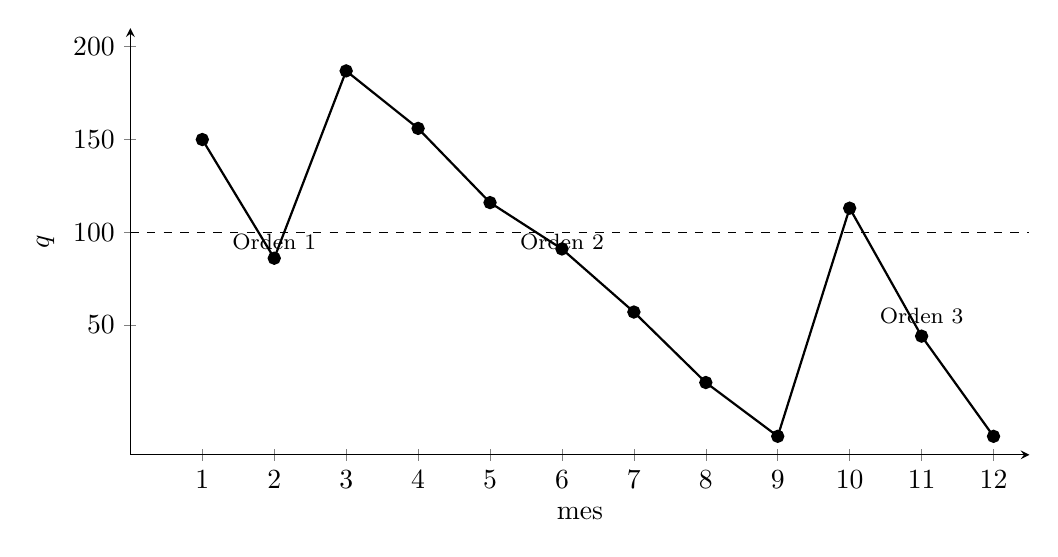
\begin{tikzpicture}
\begin{axis}[
  width=13cm, height=7cm,
  xlabel={mes}, ylabel={$q$},
  xmin=0, xmax=12.5, ymin=-20, ymax=210,
  xtick={1,2,3,4,5,6,7,8,9,10,11,12},
  ytick={50,100,150,200},
  axis lines=left,
]
\addplot[thick,mark=*] coordinates {
 (1,150)(2,86)(3,187)(4,156)(5,116)(6,91)(7,57)(8,19)(9,-10)(10,113)(11,44)(12,-10)
};
\addplot[dashed,domain=0:12.5]{100};
\node at (axis cs:2,95){\footnotesize Orden 1};
\node at (axis cs:6,95){\footnotesize Orden 2};
\node at (axis cs:11,55){\footnotesize Orden 3};
\node[right] at (axis cs:12.5,100){$R$};
\end{axis}
\end{tikzpicture}
\caption*{\textbf{Figura 5.2.} Simulación para un año de operación del sistema de inventarios.}
\end{figure}

\begin{table}[H]
\centering
\caption*{\textbf{Tabla 5.7.} Simulación manual del sistema de inventarios $(q=200,\ R=100)$.}
\begin{tabular}{cccccccc}
\toprule
\multirow{2}{*}{Mes} & Inventario & Número & Demanda & Inventario & \multirow{2}{*}{Faltante} & \multirow{2}{*}{Orden} & Inventario \\
 & inicial & aleatorio & ajustada & final & & & mensual promedio \\
\midrule
1  & 150 & 0.74022 & 64 & 86  &    & 1 & 118 \\
2  & 86  & 0.65741 & 52 & 34  &    &   & 60  \\
3  & 234 & 0.66083 & 47 & 187 &    &   & 211 \\
4  & 187 & 0.08355 & 31 & 156 &    &   & 172 \\
5  & 156 & 0.55121 & 40 & 116 &    &   & 136 \\
6  & 116 & 0.00911 & 25 & 91  &    & 2 & 104 \\
7  & 91  & 0.14060 & 34 & 57  &    &   & 74  \\
8  & 57  & 0.14845 & 38 & 19  &    &   & 38  \\
9  & 19  & 0.41839 & 48 & 0   & 29 &   & 4$^{*}$ \\
10 & 171 & 0.39685 & 58 & 113 &    &   & 142 \\
11 & 113 & 0.74416 & 69 & 44  &    & 3 & 79  \\
12 & 40  & 0.53152 & 70 & 0   & 30 &   & 11$^{**}$ \\
\bottomrule
\end{tabular}

\vspace{4pt}
{\footnotesize
$^{*}\ 4=\dfrac{19}{2}\left(\dfrac{19}{48}\right)$
\qquad
$^{**}\ 11=\dfrac{40}{2}\left(\dfrac{40}{70}\right)$}
\end{table}

\begin{table}[H]
\centering
\caption*{\textbf{Tabla 5.8.} Costos totales anuales del sistema de inventario.}
\begin{tabular}{cccc}
\toprule
Costo de ordenar & Costo de llevar inventario & Costo de faltante & Costo total \\
\midrule
$3(100)=\$300$ & $1149(1.67)=\$1{,}918$ & $59(50)=\$2{,}950$ & \$5{,}168 \\
\bottomrule
\end{tabular}
\end{table}

Si se simulan varios años más (30 por ejemplo), se podría obtener el costo
total promedio anual asociado a los valores mencionados de decisión
$(q=200, R=100)$. Sin embargo, lo importante es aplicar una metodología que
progresivamente vaya mejorando los valores de las variables de decisión
hasta determinar sus valores óptimos. Para este propósito, el algoritmo de
Hooke y Jeeaves$^{*}$ será aplicado. De acuerdo a este algoritmo, primero
hay que seleccionar valores iniciales apropiados de las variables de
decisión. Después, hay que obtener el costo total relacionado a estos
valores. En seguida, se usa esta información para mejorar los valores de las
variables de decisión. Esta iteración será repetida hasta que los valores
óptimos de las variables de decisión hayan sido encontrados. La tabla 5.12
muestra todas las iteraciones que resultan de aplicar este algoritmo. En
esta tabla se puede observar que los valores óptimos de las variables de
decisión son: $q=173$ y $R=163$, lo cual produce un costo total promedio
anual de \$3,245.

{\footnotesize $^{*}$Para entender los detalles de este algoritmo, ver
Phillips, Ravindran, Solberg, \emph{Operation Research Principles and
Practice}, John Wiley, 1976.}

\begin{table}[H]
\centering
\caption*{\textbf{Tabla 5.9.} Método de la transformada inversa para simular valores de la demanda}
\begin{tabular}{ll}
Si $0.000 \le R < 0.010$, entonces $x=35$ & Si $0.359 \le R < 0.424$, entonces $x=48$ \\
Si $0.010 \le R < 0.025$, entonces $x=36$ & Si $0.424 \le R < 0.494$, entonces $x=49$ \\
Si $0.025 \le R < 0.045$, entonces $x=37$ & Si $0.494 \le R < 0.574$, entonces $x=50$ \\
Si $0.045 \le R < 0.065$, entonces $x=38$ & Si $0.574 \le R < 0.649$, entonces $x=51$ \\
Si $0.065 \le R < 0.087$, entonces $x=39$ & Si $0.649 \le R < 0.719$, entonces $x=52$ \\
Si $0.087 \le R < 0.110$, entonces $x=40$ & Si $0.719 \le R < 0.784$, entonces $x=53$ \\
Si $0.110 \le R < 0.135$, entonces $x=41$ & Si $0.784 \le R < 0.844$, entonces $x=54$ \\
Si $0.135 \le R < 0.162$, entonces $x=42$ & Si $0.844 \le R < 0.894$, entonces $x=55$ \\
Si $0.162 \le R < 0.190$, entonces $x=43$ & Si $0.894 \le R < 0.934$, entonces $x=56$ \\
Si $0.190 \le R < 0.219$, entonces $x=44$ & Si $0.934 \le R < 0.964$, entonces $x=57$ \\
Si $0.219 \le R < 0.254$, entonces $x=45$ & Si $0.964 \le R < 0.980$, entonces $x=58$ \\
Si $0.254 \le R < 0.299$, entonces $x=46$ & Si $0.980 \le R < 0.995$, entonces $x=59$ \\
Si $0.299 \le R < 0.359$, entonces $x=47$ & Si $0.995 \le R \le 1.000$, entonces $x=60$ \\
\end{tabular}
\end{table}

\begin{table}[H]
\centering
\caption*{\textbf{Tabla 5.10.} Método de la transformada inversa para simular los tiempos de entrega}
\begin{tabular}{l}
Si $0.00 \le R < 0.30$, entonces $x=1$ mes \\
Si $0.30 \le R < 0.70$, entonces $x=2$ meses \\
Si $0.70 \le R \le 1.00$, entonces $x=3$ meses \\
\end{tabular}
\end{table}

\bigskip
\noindent\emph{Nota:} El texto de este capítulo hace referencia a un
problema adicional de sistema de colas (descarga de camiones en un almacén),
con distribuciones de probabilidad para: cantidad de camiones esperando al
abrir el almacén, tiempo entre llegadas y tiempo de servicio para equipos de
3, 4, 5 y 6 personas. A continuación se reproducen esas distribuciones y las
tablas de simulación asociadas.

\begin{table}[H]
\centering
\caption*{Camiones esperando al abrir el almacén}
\begin{tabular}{cc}
\toprule
Cantidad de camiones & Probabilidad \\
\midrule
0 & 0.50 \\
1 & 0.25 \\
2 & 0.15 \\
3 & 0.10 \\
\bottomrule
\end{tabular}
\end{table}

\begin{table}[H]
\centering
\caption*{Distribución del tiempo entre llegadas}
\begin{tabular}{cc}
\toprule
Tiempo entre llegadas (minutos) & Probabilidad \\
\midrule
20 & 0.02 \\
25 & 0.08 \\
30 & 0.12 \\
35 & 0.25 \\
40 & 0.20 \\
45 & 0.15 \\
50 & 0.10 \\
55 & 0.05 \\
60 & 0.03 \\
\bottomrule
\end{tabular}
\end{table}

\begin{table}[H]
\centering
\caption*{Distribuciones del tiempo de servicio para diferentes tamaños de equipo}
\begin{tabular}{cccc}
\toprule
\multicolumn{2}{c}{Equipo de tres personas} & \multicolumn{2}{c}{Equipo de cuatro personas} \\
Tiempo (min) & Probabilidad & Tiempo (min) & Probabilidad \\
\midrule
20 & 0.05 & 15 & 0.05 \\
25 & 0.10 & 20 & 0.15 \\
30 & 0.20 & 25 & 0.20 \\
35 & 0.25 & 30 & 0.20 \\
40 & 0.12 & 35 & 0.15 \\
45 & 0.10 & 40 & 0.12 \\
50 & 0.08 & 45 & 0.08 \\
55 & 0.06 & 50 & 0.04 \\
60 & 0.04 & 55 & 0.01 \\
\bottomrule
\end{tabular}
\end{table}

\begin{table}[H]
\centering
\begin{tabular}{cccc}
\toprule
\multicolumn{2}{c}{Equipo de cinco personas} & \multicolumn{2}{c}{Equipo de seis personas} \\
Tiempo (min) & Probabilidad & Tiempo (min) & Probabilidad \\
\midrule
10 & 0.10 & 5  & 0.12 \\
15 & 0.18 & 10 & 0.15 \\
20 & 0.22 & 15 & 0.26 \\
25 & 0.18 & 20 & 0.15 \\
30 & 0.10 & 25 & 0.12 \\
35 & 0.08 & 30 & 0.08 \\
40 & 0.06 & 35 & 0.06 \\
45 & 0.05 & 40 & 0.04 \\
50 & 0.03 & 45 & 0.02 \\
\bottomrule
\end{tabular}
\end{table}

Si todo el equipo se considera como un servidor, ¿cuál es el tamaño óptimo
del equipo?

El análisis de sistemas de colas frecuentemente ilustra la dificultad de
construir un modelo matemático que contenga todos los elementos presentes en
el sistema. Generalmente, los modelos de colas asumen que el tiempo entre
llegadas y el tiempo de servicio siguen una distribución exponencial.
También, estos modelos asumen que la cantidad de clientes que llegan al
sistema por unidad de tiempo y la cantidad de clientes que el sistema sirve
por unidad de tiempo siguen una distribución poisson. Además de las
anteriores suposiciones, estos modelos generalmente asumen que: 1) La fuente
que alimenta al sistema es de tamaño infinito; 2) El sistema ha alcanzado el
estado estable; 3) La disciplina de servicio es primeras
entradas---primeras salidas; 4) Los clientes que llegan al sistema se unen a
la cola; 5) Los clientes que están en la cola, permanecerán en ella hasta
que sean servidos; 6) Los clientes llegan en forma individual y 7) Las
salidas del sistema son en forma individual. Estas suposiciones generalmente
originan que las decisiones que se toman con base en estos modelos no sean
confiables.

En muchas situaciones, sin embargo, el sistema de colas puede tener
características especiales importantes. Puede tener etapas transientes y de
estado estable, puede ser dependiente, o formar parte de un grupo de
facilidades independientes. Puede tener prioridades de servicio, o algunos
clientes que llegan al sistema cuando la cola es excesivamente grande pueden
rehusar entrar al sistema. También, puede ser que la fuente que alimenta al
sistema sea finita. La exclusión de tales características especiales puede
distorsionar la naturaleza verdadera del sistema, por lo cual deberán ser
consideradas en la modelación del mismo.

Si hay varias características especiales importantes, una modelación
matemática completa resultaría difícil o casi imposible. En tales
situaciones, el análisis completo del sistema puede ser logrado a través del
uso de la técnica de simulación.

A través de las operaciones del turno nocturno, el tiempo entre llegadas y
el tiempo de servicio son obtenidos utilizando números aleatorios del
apéndice. Después de cada evento, el \emph{reloj de la simulación} es
actualizado. Tan pronto como algún servicio sea terminado después de las 3
A.M., el personal dispondrá de media hora para tomar sus alimentos. Para
este caso resultó de 3.15 a 3.45 A.M. Para descargar el último camión, el
cual llegó a las 6.55 A.M., el personal tuvo que trabajar 10 minutos de
tiempo extra. Por consiguiente, los costos totales que se incurren en este
primer turno simulado son:

\begin{align*}
\text{Salarios} &= \text{Tiempo normal} + \text{tiempo extra} \\
&= 3(8)(25) + 37.50(3)(1/6) \\
&= \$618.75. \\[6pt]
\text{Espera} &= \text{Operación del almacén} + \text{espera del camión} \\
&= 500(8.67) + 100(6.42) \\
&= \$4{,}977. \\[6pt]
\text{Costo total} &= 618.75 + 4{,}977 = \$5{,}595.75
\end{align*}

\begin{table}[H]
\centering
\caption*{\textbf{Tabla 5.13.} Método de la transformada inversa para simular los camiones que esperan al empezar a operar el almacén.}
\begin{tabular}{l}
Si $0.00 \le R < 0.50$, entonces $x=0$ \\
Si $0.50 \le R < 0.75$, entonces $x=1$ \\
Si $0.75 \le R < 0.90$, entonces $x=2$ \\
Si $0.90 \le R < 1.00$, entonces $x=3$ \\
\end{tabular}
\end{table}

\begin{table}[H]
\centering
\caption*{\textbf{Tabla 5.14.} Método de la transformada inversa para simular el tiempo entre llegadas.}
\begin{tabular}{l}
Si $0.00 \le R < 0.02$, entonces $x=20$ \\
Si $0.02 \le R < 0.10$, entonces $x=25$ \\
Si $0.10 \le R < 0.22$, entonces $x=30$ \\
Si $0.22 \le R < 0.47$, entonces $x=35$ \\
Si $0.47 \le R < 0.67$, entonces $x=40$ \\
Si $0.67 \le R < 0.82$, entonces $x=45$ \\
Si $0.82 \le R < 0.92$, entonces $x=50$ \\
Si $0.92 \le R < 0.97$, entonces $x=55$ \\
Si $0.97 \le R \le 1.00$, entonces $x=60$ \\
\end{tabular}
\end{table}

\begin{table}[H]
\centering
\caption*{\textbf{Tabla 5.15.} Método de la transformada inversa para simular el tiempo de servicio (equipo de 3 personas).}
\begin{tabular}{l}
Si $0.00 \le R < 0.05$, entonces $x=20$ \\
Si $0.05 \le R < 0.15$, entonces $x=25$ \\
Si $0.15 \le R < 0.35$, entonces $x=30$ \\
Si $0.35 \le R < 0.60$, entonces $x=35$ \\
Si $0.60 \le R < 0.72$, entonces $x=40$ \\
Si $0.72 \le R < 0.82$, entonces $x=45$ \\
Si $0.82 \le R < 0.90$, entonces $x=50$ \\
Si $0.90 \le R < 0.96$, entonces $x=55$ \\
Si $0.96 \le R \le 1.00$, entonces $x=60$ \\
\end{tabular}
\end{table}

\begin{table}[H]
\centering
\caption*{\textbf{Tabla 5.16.} Método de la transformada inversa para simular el tiempo de servicio (equipo de 4 personas).}
\begin{tabular}{l}
Si $0.00 \le R < 0.05$, entonces $x=15$ \\
Si $0.05 \le R < 0.20$, entonces $x=20$ \\
Si $0.20 \le R < 0.40$, entonces $x=25$ \\
Si $0.40 \le R < 0.60$, entonces $x=30$ \\
Si $0.60 \le R < 0.75$, entonces $x=35$ \\
Si $0.75 \le R < 0.87$, entonces $x=40$ \\
Si $0.87 \le R < 0.95$, entonces $x=45$ \\
Si $0.95 \le R < 0.99$, entonces $x=50$ \\
Si $0.99 \le R \le 1.00$, entonces $x=55$ \\
\end{tabular}
\end{table}

\begin{table}[H]
\centering
\caption*{\textbf{Tabla 5.17.} Método de la transformada inversa para simular el tiempo de servicio (equipo de 5 personas).}
\begin{tabular}{l}
Si $0.00 \le R < 0.10$, entonces $x=10$ \\
Si $0.10 \le R < 0.28$, entonces $x=15$ \\
Si $0.28 \le R < 0.50$, entonces $x=20$ \\
Si $0.50 \le R < 0.68$, entonces $x=25$ \\
Si $0.68 \le R < 0.78$, entonces $x=30$ \\
Si $0.78 \le R < 0.86$, entonces $x=35$ \\
Si $0.86 \le R < 0.92$, entonces $x=40$ \\
Si $0.92 \le R < 0.97$, entonces $x=45$ \\
Si $0.97 \le R \le 1.00$, entonces $x=50$ \\
\end{tabular}
\end{table}

\begin{table}[H]
\centering
\caption*{\textbf{Tabla 5.18.} Método de la transformada inversa para simular el tiempo de servicio (equipo de 6 personas).}
\begin{tabular}{l}
Si $0.00 \le R < 0.12$, entonces $x=5$ \\
Si $0.12 \le R < 0.27$, entonces $x=10$ \\
Si $0.27 \le R < 0.53$, entonces $x=15$ \\
Si $0.53 \le R < 0.68$, entonces $x=20$ \\
Si $0.68 \le R < 0.80$, entonces $x=25$ \\
Si $0.80 \le R < 0.88$, entonces $x=30$ \\
Si $0.88 \le R < 0.94$, entonces $x=35$ \\
Si $0.94 \le R < 0.98$, entonces $x=40$ \\
Si $0.98 \le R \le 1.00$, entonces $x=45$ \\
\end{tabular}
\end{table}

Aunque esta es la simulación de un turno, los resultados son significativos.
Los camiones esperan demasiado tiempo. Los costos de espera son mucho
mayores que los salarios percibidos por el personal. A partir de estos
resultados, podría pensarse que incrementando el número de personas
encargadas de descargar los camiones, el costo total promedio por turno se
reduciría. Veamos qué pasa si el tamaño del equipo se incrementa a 4
personas. Para este propósito, la tabla 5.20 muestra los resultados
obtenidos en una simulación manual de un turno de operación. Para este nuevo
tamaño de equipo, los costos totales que se incurren en el primer turno
simulado son:

\begin{align*}
\text{Salarios} &= 4(8)(25) + 37.50(4)(1/4) = \$837.50. \\[6pt]
\text{Espera} &= 500(8.75) + 100(0.83) = \$4{,}458. \\[6pt]
\text{Costo total} &= 837.50 + 4{,}458 = \$5{,}295.50
\end{align*}

De los resultados anteriores, podría pensarse que 4 trabajadores es más
económico que tres trabajadores. Sin embargo, considerar adecuadamente las
variaciones en los resultados obtenidos con diferentes tamaños de equipo,
requiere realizar un gran número de simulaciones.

Si se varía el tamaño del equipo y se simulan varios turnos, entonces, es
posible determinar el tamaño del equipo para el cual los costos totales son
mínimos. La tabla 21 muestra los resultados que se obtienen al simular la
operación del almacén durante 60 turnos. Para estas simulaciones se
consideraron tamaños de equipo de 3, 4, 5 y 6 personas. Como se puede
apreciar en esta tabla, el tamaño óptimo del equipo es de 6 personas. Esto
significa, que la forma más económica de operar el almacén es con un equipo
de 6 personas.

\begin{table}[H]
\centering
\caption*{\textbf{Tabla 5.19.} Simulación de las operaciones de descarga durante un turno (equipo de 3 personas).}
\small
\resizebox{\textwidth}{!}{%
\begin{tabular}{ccccccccc}
\toprule
Número & Tiempo entre & Tiempo de & Iniciación & Número & Tiempo de & Terminación & Ocio del & Tiempo de espera / Long. \\
aleatorio & llegadas & llegada & del servicio & aleatorio & servicio & del servicio & personal & del camión / cola \\
\midrule
0.48355 & --    & 11:00 & 11:00 & 0.83761 & 50 & 11:50 & --  & -- / 1 \\
0.98977 & 40    & 11:40 & 11:50 & 0.14387 & 25 & 12:15 & --  & 10 / 1 \\
0.06533 & 60    & 12:40 & 12:40 & 0.51321 & 35 & 1:15  & 25  & -- / 0 \\
0.45128 & 25    & 1:05  & 1:15  & 0.72472 & 45 & 2:00  & --  & 10 / 1 \\
0.15486 & 35    & 1:40  & 2:00  & 0.05466 & 25 & 2:25  & --  & 20 / 1 \\
0.19241 & 30    & 2:10  & 2:25  & 0.84609 & 50 & 3:15  & --  & 15 / 1 \\
0.15997 & 30    & 2:40  & 3:15  & 0.29735 & 30 & 4:15  & --  & 65 / 2 \\
0.67940 & 30    & 3:10  & 4:15  & 0.59076 & 35 & 4:50  & --  & 65 / 2 \\
0.90872 & 45    & 3:55  & 4:50  & 0.76355 & 45 & 5:35  & --  & 55 / 2 \\
0.58997 & 50    & 4:45  & 5:35  & 0.29549 & 30 & 6:05  & --  & 50 / 2 \\
0.68691 & 40    & 5:25  & 6:05  & 0.61958 & 40 & 6:45  & --  & 40 / 2 \\
0.73488 & 45    & 6:10  & 6:45  & 0.17267 & 30 & 7:15  & --  & 35 / 1 \\
        & 45    & 6:55  & 7:15  & 0.10061 & 25 & 7:40  & --  & 20 / 1 \\
\bottomrule
\end{tabular}}

\vspace{2pt}
{\footnotesize \emph{Nota:} En esta simulación solamente se simuló la
llegada de 12 camiones, puesto que el camión número 13, de acuerdo al número
aleatorio generado, llega después de las 7:00 A.M.}
\end{table}

\begin{table}[H]
\centering
\caption*{\textbf{Tabla 5.20.} Simulación de las operaciones de descarga durante un turno (equipo de 4 personas).}
\small
\resizebox{\textwidth}{!}{%
\begin{tabular}{ccccccccc}
\toprule
Número & Tiempo entre & Tiempo de & Iniciación & Número & Tiempo de & Terminación & Ocio del & Tiempo de espera / Long. \\
aleatorio & llegadas & llegada & del servicio & aleatorio & servicio & del servicio & personal & del camión / cola \\
\midrule
0.68971 & --    & 11:00 & 11:00 & 0.11403 & 20 & 11:20 & --  & -- / 1 \\
0.18477 & 45    & 11:45 & 11:45 & 0.65622 & 35 & 12:20 & 25  & -- / 0 \\
0.14707 & 30    & 12:15 & 12:20 & 0.93997 & 45 & 1:05  & --  & 5 / 1 \\
0.83745 & 30    & 12:45 & 1:05  & 0.22567 & 25 & 1:30  & --  & 20 / 1 \\
0.16930 & 50    & 1:35  & 1:35  & 0.33361 & 25 & 2:00  & 5   & -- / 0 \\
0.20368 & 30    & 2:05  & 2:05  & 0.07126 & 20 & 2:25  & 5   & -- / 0 \\
0.41196 & 30    & 2:35  & 2:35  & 0.37480 & 25 & 3:00  & 10  & -- / 0 \\
0.66919 & 35    & 3:10  & 3:30  & 0.31678 & 25 & 3:55  & --  & 20 / 1 \\
0.35352 & 40    & 3:50  & 3:55  & 0.54131 & 30 & 4:25  & --  & 5 / 1 \\
0.79982 & 35    & 4:25  & 4:25  & 0.68416 & 35 & 5:00  & --  & -- / 0 \\
0.46850 & 45    & 5:10  & 5:10  & 0.52326 & 30 & 5:40  & 10  & -- / 0 \\
0.69248 & 35    & 5:45  & 5:45  & 0.93460 & 45 & 6:30  & 5   & -- / 0 \\
0.04013 & 45    & 6:35  & 6:35  & 0.31792 & 25 & 7:00  & 5   & -- / 0 \\
        & 25    & 7:00  & 7:00  & 0.87315 & 45 & 7:45  & --  & -- / 0 \\
\bottomrule
\end{tabular}}

\vspace{2pt}
{\footnotesize \emph{Nota:} También esta simulación es igual que en la tabla
anterior, el último camión simulado llega después de las 7:00 A.M.}
\end{table}

\begin{table}[H]
\centering
\caption*{\textbf{Tabla 21.} Simulación por computadora del sistema de colas durante 60 turnos y considerando diferentes tamaños de equipo.}
\begin{tabular}{cccccc}
\toprule
Tamaño del & Salario & Salario & Ocio del & Operación del & Costos \\
equipo & normal & extra & camión & almacén & totales \\
\midrule
3 & \$600   & \$421 & \$2{,}261 & \$6{,}121 & \$9{,}403 \\
4 & 800     & 335   & 1{,}202   & 5{,}367   & 7{,}704 \\
5 & 1{,}000 & 165   & 455       & 4{,}689   & 6{,}309 \\
6 & 1{,}200 & 47    & 125       & 4{,}354   & 5{,}720 \\
\bottomrule
\end{tabular}
\end{table}

%==========================================================
\section*{PROBLEMAS}

\begin{description}[leftmargin=1.2cm,style=nextline]

\item[5.1.] El famoso juego 7-11, requiere que el jugador lance dos dados
una o más veces hasta tomar la decisión de que se gana o se pierde el juego.
El juego se gana si en el primer lanzamiento los dados suman 7 u 11, ó
aparece un 4, 5, 6, 8, 9 ó 10 en el primer lanzamiento y la misma suma
reaparece antes de que aparezca un 7. Por otra parte, el juego se pierde si
en el primer lanzamiento los dados suman 2, 3 ó 12, ó aparece un 4, 5, 6, 8,
9 ó 10 en el primer lanzamiento y luego sale un 7 antes de que se repita el
primer lanzamiento. Si el valor de la apuesta es de \$1, y la ganancia cada
vez que se gana un juego es de \$1, ¿cuál sería la probabilidad de quiebra si
la cantidad inicial disponible es de \$20? (Asuma que el juego también se
termina cuando se acumulan \$50.)

\item[5.2.] En el famoso juego de la ruleta, existen muchas opciones para
apostar. Una de ellas consiste en apostarle al color rojo o al color negro.
En el tablero de la ruleta existen 10 números rojos, 10 números negros y 2
números verdes (cero y doble cero). Si un jugador apuesta a un color y el
color aparece, él o ella gana la cantidad apostada. Si otro color aparece,
el jugador pierde la cantidad apostada. Si el color verde aparece, la rueda
de la ruleta se vuelve a girar hasta que el color rojo o negro aparezca. Si
este color es el color que se apostó, el jugador no gana ni pierde. De otra
forma, se pierde la cantidad apostada.

Dos jugadores usan diferentes estrategias. Un jugador simplemente apuesta \$1
al color rojo cada vez. El otro jugador empieza apostando un \$1 al color
rojo. Si él gana, él apuesta otro \$1. Sin embargo, si él pierde, él apuesta
\$2 la próxima vez. Si él pierde otra vez, él apuesta \$4. Este jugador puede
continuar doblando la apuesta hasta un límite de \$500.00. Si él pierde esta
apuesta de \$500, él empieza apostando nuevamente \$1. Si cada jugador inicia
el juego con \$200, ¿cuál cree usted que es la mejor estrategia?

\item[5.3.] Una compañía de renta de autos, está tratando de determinar el
número óptimo de autos a comprar. El costo promedio anual de un auto es de
\$75,000. Además, esta compañía ha recopilado las siguientes probabilidades
de operación:

\begin{center}
\begin{tabular}{lccccc}
Número de autos rentados por día & 0 & 1 & 2 & 3 & 4 \\
Probabilidad & 0.10 & 0.10 & 0.25 & 0.30 & 0.25 \\[6pt]
Número de días rentados por auto & 1 & 2 & 3 & 4 & \\
Probabilidad & 0.40 & 0.35 & 0.15 & 0.10 & \\
\end{tabular}
\end{center}

Si la renta diaria por auto es de \$350, el costo de no tener un auto
disponible cuando se está solicitando es de \$200, y el costo de tener un
carro ocioso durante un día es de \$50, ¿cuál es la cantidad de autos que
debería comprar la compañía? (Asuma que un auto que se renta por un día está
disponible al día siguiente. También, asuma 365 días de operación al año.)

\item[5.4.] Una flecha será ensamblada en un cojinete como se muestra a
continuación:

\begin{center}
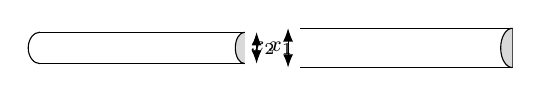
\begin{tikzpicture}[scale=1]
  \draw (0,0.2) -- (2.6,0.2) -- (2.6,-0.2) -- (0,-0.2);
  \draw (0,0.2) arc (90:270:0.15 and 0.2);
  \draw[fill=gray!30] (2.6,0.2) arc (90:270:0.12 and 0.2);
  \draw[{Latex}-{Latex}] (2.75,0.2) -- (2.75,-0.2);
  \node[right] at (2.78,0) {\footnotesize $x_1$};
  \draw (3.3,0.25) -- (6,0.25) -- (6,-0.25) -- (3.3,-0.25);
  \draw[fill=gray!30] (6,0.25) arc (90:270:0.15 and 0.25);
  \draw[{Latex}-{Latex}] (3.15,0.25) -- (3.15,-0.25);
  \node[left] at (3.12,0) {\footnotesize $x_2$};
\end{tikzpicture}
\end{center}

Si $x_1$ sigue una distribución normal con media 1.5 y variancia 0.0016, y
$X_2$ sigue esta misma distribución con media 1.48 y variancia 0.0009,
determine:
\begin{enumerate}[label=\alph*)]
\item La probabilidad de que haya interferencia.
\item El número de veces que es necesario simular el experimento, si se
quiere que la probabilidad de interferencia estimada difiera de su valor
verdadero en menos de 0.01, con un nivel de seguridad del 95\%.
\end{enumerate}

\item[5.5.] La demanda diaria de un cierto artículo está regida por una
distribución binomial con parámetros $n=6$ y $\theta=1/2$. El tiempo de
entrega en días es una variable aleatoria poisson con $\lambda=3$. El costo
de mantener una unidad en inventario es de \$1 por día, el costo del faltante
es de \$10 por unidad, y el costo de ordenar es de \$50 por orden. Se desea
comparar dos políticas para llevar el inventario: 1) Ordenar cada 8 días
hasta tener 30 artículos en inventario y 2) Ordenar hasta 30 artículos
cuando el nivel del inventario sea menor o igual a 10. Si se asume que las
unidades faltantes en un ciclo son surtidas por la nueva orden que arriba en
el próximo ciclo, ¿cuál de las dos políticas descritas es más económica?

\item[5.6.] Una compañía tiene un problema de mantenimiento con cierto
equipo, que contiene 4 componentes electrónicos idénticos que son la causa
del mismo, el cual consiste en que los componentes fallan frecuentemente,
forzando a que el equipo se desconecte mientras se hace la reposición. Lo
que se ha venido haciendo es reemplazar los componentes solamente cuando se
descomponen. Sin embargo, existe una nueva proposición de hacer el reemplazo
de los cuatro componentes cuando falle cualesquiera de ellos, con objeto de
reducir la frecuencia de desconexión del equipo.

El tiempo de vida de un componente está normalmente distribuido con media de
600 horas y desviación estándar de 100 horas. También se sabe que es
necesario desconectar el equipo 1 hora si se reemplaza un componente y 2
horas si se reemplazan los 4. Un componente nuevo cuesta \$200 y se incurre
en un costo de \$100 por hora cada vez que se desconecta el equipo.

Determine cuál de las dos políticas anteriores es más económica (Simule la
operación del equipo durante 20,000 horas).

\item[5.7.] Un vendedor de revistas compra mensualmente una revista el día
primero de cada mes. El costo de cada ejemplar es de \$1.50. La demanda de
esta revista en los primeros 10 días del mes sigue la siguiente distribución
de probabilidad:

\begin{center}
\begin{tabular}{lccccccc}
Demanda & 5 & 6 & 7 & 8 & 9 & 10 & 11 \\
Probabilidad & 0.05 & 0.05 & 0.10 & 0.15 & 0.25 & 0.25 & 0.15 \\
\end{tabular}
\end{center}

Al final del décimo día, el vendedor puede regresar cualquier cantidad al
proveedor, quien se las pagará a \$0.90 el ejemplar, o comprar más a \$1.20 el
ejemplar. La demanda en los siguientes 20 días está dada por la siguiente
distribución de probabilidad:

\begin{center}
\begin{tabular}{lccccc}
Demanda & 4 & 5 & 6 & 7 & 8 \\
Probabilidad & 0.15 & 0.20 & 0.30 & 0.20 & 0.15 \\
\end{tabular}
\end{center}

Al final del mes, el vendedor puede regresar al proveedor las revistas que le
sobren, las cuales se le pagarán a \$0.60 el ejemplar. Finalmente, se asume
que después de un mes ya no existe demanda por parte del público, puesto que
para ese entonces ya habrá aparecido el nuevo número de la revista. Si el
precio al público es de \$2 por ejemplar, determine la política óptima de
compra.

\item[5.8.] Una compañía desea entrar en un nuevo negocio cuya inversión
inicial requerida y los ingresos netos anuales después de impuestos están
distribuidos como sigue:

\begin{center}
\begin{tabular}{ll}
Inversión inicial & $\sim N(\mu=100{,}000;\ \sigma=5{,}000)$ \\
Flujo neto del período $t$ & $\sim N(\mu=30{,}000;\ \sigma=3{,}000)$ \\
\end{tabular}
\end{center}

Si la administración ha establecido que un proyecto de inversión será
emprendido si $\Prob\{\text{TIR} > \text{TREMA}\} \ge 0.90$, y la TREMA es de
30\%, ¿debería la compañía $X$ aceptar este nuevo proyecto de inversión?
(Asuma un horizonte de planeación de 5 años y un valor de rescate al término
de este tiempo de cero).

\item[5.9.] Una compañía está interesada en analizar un negocio cuya
inversión inicial sigue la siguiente distribución triangular:

\begin{center}
\begin{tabular}{ccc}
Estimación pesimista & Estimación más probable & Estimación optimista \\
$-130{,}000$ & $-100{,}000$ & $-80{,}000$ \\
\end{tabular}
\end{center}

Esta inversión tiene una vida fiscal de 5 años, y un valor de rescate al
término de este período distribuido triangularmente:

\begin{center}
\begin{tabular}{ccc}
Estimación pesimista & Estimación más probable & Estimación optimista \\
16{,}000 & 20{,}000 & 26{,}000 \\
\end{tabular}
\end{center}

La tasa de inflación en los próximos cinco años, está regida por la siguiente
distribución triangular:

\begin{center}
\begin{tabular}{ccc}
Estimación pesimista & Estimación más probable & Estimación optimista \\
25\% & 20\% & 15\% \\
\end{tabular}
\end{center}

Finalmente, asuma que los ingresos netos de los próximos cinco años siguen la
siguiente distribución uniforme:

\begin{center}
\begin{tabular}{lccccc}
Año & 1 & 2 & 3 & 4 & 5 \\
\midrule
Flujos & 20{,}000 & 30{,}000 & 40{,}000 & 50{,}000 & 60{,}000 \\
Probabilidad & 1/5 & 1/5 & 1/5 & 1/5 & 1/5 \\
\end{tabular}
\end{center}

Si la tasa de impuestos es de 50\%, la TREMA de 20\%, y la alta
administración acepta un nuevo proyecto si $\Prob\{\text{VPN} > 0\} \ge 0.90$,
¿debería la compañía emprender este nuevo proyecto de inversión?

\item[5.10.] La demanda diaria y el tiempo de entrega de un cierto producto,
siguen las siguientes distribuciones de probabilidad:

\begin{center}
\begin{tabular}{cc@{\hskip 1.5cm}cc}
\multicolumn{2}{c}{} & \multicolumn{2}{c}{Tiempo de} \\
Demanda diaria & Probabilidad & entrega (días) & Probabilidad \\
\midrule
0 & 0.04 & 1 & 0.25 \\
1 & 0.06 & 2 & 0.50 \\
2 & 0.10 & 3 & 0.20 \\
3 & 0.20 & 4 & 0.05 \\
4 & 0.30 &   &      \\
5 & 0.18 &   &      \\
6 & 0.08 &   &      \\
7 & 0.03 &   &      \\
8 & 0.01 &   &      \\
\end{tabular}
\end{center}

La información con respecto a los costos relevantes es la siguiente:
\begin{center}
\begin{tabular}{ll}
Costo de ordenar    & $=$ \$50/orden \\
Costo de inventario & $=$ \$26/unidad/año \\
Costo de faltante   & $=$ \$25/unidad \\
\end{tabular}
\end{center}

Si el inventario inicial es de 15 unidades, ¿determine la cantidad óptima a
ordenar $(q)$ y el nivel óptimo de reorden $(R)$? (Asuma que se trabajan 260
días en el año.)

\item[5.11.] La demanda diaria y el tiempo de entrega de un cierto producto,
siguen las siguientes distribuciones de probabilidad:

\begin{center}
\begin{tabular}{cc@{\hskip 1.5cm}cc}
\multicolumn{2}{c}{} & \multicolumn{2}{c}{Tiempo de} \\
Demanda diaria & Probabilidad & entrega (días) & Probabilidad \\
\midrule
25 & 0.02 & 1 & 0.20 \\
26 & 0.04 & 2 & 0.30 \\
27 & 0.06 & 3 & 0.25 \\
28 & 0.12 & 4 & 0.25 \\
29 & 0.20 &   &      \\
30 & 0.24 &   &      \\
31 & 0.15 &   &      \\
32 & 0.10 &   &      \\
33 & 0.05 &   &      \\
34 & 0.02 &   &      \\
\end{tabular}
\end{center}

Si el producto no está disponible cuando es requerido, el cliente puede
esperar la llegada de un nuevo lote por un tiempo limitado, es decir, si el
cliente decide esperar 2 días y la mercancía no llega en ese tiempo,
entonces, la demanda de este cliente se considera perdida. La distribución de
probabilidad del tiempo que un cliente está dispuesto a esperar para que se
le surta su pedido, es la siguiente:

\begin{center}
\begin{tabular}{cc}
Tiempo de espera (días) & Probabilidad \\
\midrule
0 & 0.40 \\
1 & 0.20 \\
2 & 0.15 \\
3 & 0.15 \\
4 & 0.10 \\
\end{tabular}
\end{center}

La información con respecto a los costos relevantes es la siguiente:
\begin{center}
\begin{tabular}{ll}
Costo de ordenar & $=$ \$100/orden \\
Costo de inventario & $=$ \$52/unidad/año \\
Costo de faltante suponiendo que el cliente espera & $=$ \$20/unidad \\
Costo de faltante suponiendo que el cliente no espera & $=$ \$50/unidad \\
\end{tabular}
\end{center}

Si el inventario inicial es de 100 unidades, ¿determine la cantidad óptima a
ordenar $(q)$ y el nivel óptimo de reorden $(R)$? (Asuma que se trabajan 260
días en el año).

\item[5.12.] Se tiene un sistema de colas formado por dos estaciones en
serie. Los clientes atendidos en la primera estación pasan en seguida a
formar cola en la segunda. En la primera estación de servicio, la razón de
llegadas sigue una distribución poisson con media de 20 clientes por hora, y
el tiempo de servicio sigue una distribución exponencial con media de 2
minutos por persona. En la segunda estación, el tiempo de servicio está
uniformemente distribuido entre 1 y 2 minutos. Para esta información, ¿cuál
es el tiempo promedio en el sistema?, ¿cuál de las dos colas que se forman es
mayor?

\item[5.13.] Un banco emplea 3 cajeros para servir a sus clientes. Los
clientes arriban de acuerdo a un proceso poisson a una razón media de 40 por
hora. Si un cliente encuentra todos los cajeros ocupados, entonces se
incorpora a la cola que alimenta a todos los cajeros. El tiempo que dura la
transacción entre un cajero y un cliente sigue una distribución uniforme
entre 0 y 1 minuto. Para esta información, ¿cuál es el tiempo promedio en el
sistema?, ¿cuál es la cantidad promedio de clientes en el sistema?

\item[5.14.] Una tienda pequeña tiene un lote de estacionamiento con 6
lugares disponibles. Los clientes llegan en forma aleatoria de acuerdo a un
proceso poisson a una razón media de 10 clientes por hora, y se van
inmediatamente si no existen lugares disponibles en el estacionamiento. El
tiempo que un auto permanece en el estacionamiento sigue una distribución
uniforme entre 10 y 30 minutos.
\begin{enumerate}[label=\alph*)]
\item ¿Qué porcentaje de los clientes es perdido por no tener más lugares
disponibles?
\item ¿Cuál es la probabilidad de encontrar un lugar disponible en el
estacionamiento?
\item ¿Cuál es el porcentaje promedio de espacios disponibles?
\end{enumerate}

\item[5.15.] Debido a un aumento en las ventas, cierta compañía manufacturera
necesita más espacio en su fábrica. La solución que se ha propuesto es la
construcción de un nuevo depósito para almacenar los productos terminados.
Este depósito estaría localizado a 30 kilómetros del lugar donde está ubicada
la planta. Además, de acuerdo a este nuevo plan, se requiere que al final del
día se envíe al nuevo depósito, la producción terminada.

Por otra parte, se sabe de información pasada, que la producción diaria de
esta compañía, sigue la siguiente distribución de probabilidad:

\begin{center}
\begin{tabular}{cc}
Producción diaria en toneladas & Probabilidad \\
\midrule
50 - 55 & 0.10 \\
55 - 60 & 0.15 \\
60 - 65 & 0.30 \\
65 - 70 & 0.35 \\
75 - 80 & 0.08 \\
80 - 85 & 0.02 \\
\end{tabular}
\end{center}

También, se sabe que el tipo de camiones que se deben utilizar para
trasladar esta producción, tienen una capacidad media de carga de 5
toneladas. La cantidad de viajes que se pueden realizar cada día (jornada de
8 horas), depende del tiempo de carga y de descarga, como también del tiempo
que se requiere para recorrer los treinta kilómetros entre la planta y el
depósito. Consecuentemente, la cantidad de producto terminado que un camión
puede trasladar de la planta al depósito, es una variable aleatoria cuya
distribución de probabilidad es la siguiente:

\begin{center}
\begin{tabular}{cc}
Toneladas diarias trasladadas por camión & Probabilidad \\
\midrule
4.0 - 4.5 & 0.30 \\
4.5 - 5.0 & 0.40 \\
5.0 - 5.5 & 0.20 \\
5.5 - 6.0 & 0.10 \\
\end{tabular}
\end{center}

Si la cantidad diaria producida es mayor que la cantidad que puede trasladar
la flotilla de camiones, el excedente es enviado a través de otra compañía
transportista a un costo de \$100 por tonelada. Además, el costo promedio
anual de un nuevo camión es de \$100,000. Si se trabajan 250 días en el año,
¿cuál es el número óptimo de camiones que esta compañía debe de adquirir?

\item[5.16.] Una cierta compañía posee un gran número de máquinas en uso. El
tiempo que dura en operación cada una de estas máquinas, sigue la siguiente
distribución de probabilidad:

\begin{center}
\begin{tabular}{cc}
Tiempo entre descomposturas (horas) & Probabilidad \\
\midrule
6 - 8   & 0.10 \\
8 - 10  & 0.15 \\
10 - 12 & 0.24 \\
12 - 14 & 0.26 \\
16 - 18 & 0.18 \\
18 - 20 & 0.07 \\
\end{tabular}
\end{center}

El tiempo que un operador se tarda en reparar una máquina, sigue la siguiente
distribución de probabilidad:

\begin{center}
\begin{tabular}{cc}
Tiempo de reparación (horas) & Probabilidad \\
\midrule
2 - 4   & 0.15 \\
4 - 6   & 0.25 \\
6 - 8   & 0.30 \\
8 - 10  & 0.20 \\
10 - 12 & 0.10 \\
\end{tabular}
\end{center}

Si el costo de tener una máquina ociosa durante una hora es de \$500, y el
salario por hora para este tipo de operarios es de \$50, ¿cuántas máquinas se
deben asignar a cada mecánico para que las atienda?

\end{description}

\end{document}
